\chapter{Planning}

\section*{ }
To finally deliver the final output, we went into a 4 phases process:

\section{The Benchmarking Phase}
This is the phase that we decide what to implement, where to deploy them and why we have took those technical decisions. 
\bigskip

As Already mentioned, 3 main components will be developed on blockchain, still to decide which blockchain to work with, since there is many to choose from. So based on what criteria we will choose the technology and which excels at which, This is the goal of this phase.


\section{The Research Phase}
This is the phase where we look up public implementations and best practices. because it is our first time working with this domain, the best first steps we can take is to see a ready work, and decompose it and analyse its architecture, dependencies, tests.. Then we take what we learned to be the foundation to build our specific project.


\section{Smart Contracts Implementation}
This is the phase where we start writing code. For each part of the project we write all the necessary smart contracts and Factories and libraries, we test them by writing Unit tests in a Typescript, and try to target specific scenarios to make sure that our contracts work the way we intended to be. As a final addition we try to refactor the code and add as much optimizations as possible because smart contracts can consume much more gaz fees for simple instructions, the most important part of writing contracts is that it consume less, not perform better.

\section{The Demo Phase}
Finally, after making sure our contracts work perfectly, it is time to put them into real world test, where we deploy them into a test network (which is a compatible blockchain with fake money, just to test the contracts before shipping them to production), and build simple frontend apps to consume from the deployed contracts, and eventually present them in a demo and showcase all the promised features.
\bigskip

Here is a Gantt Chart demonstrating the process we planned from start to demo.

\rotatebox[origin=c]{-90}{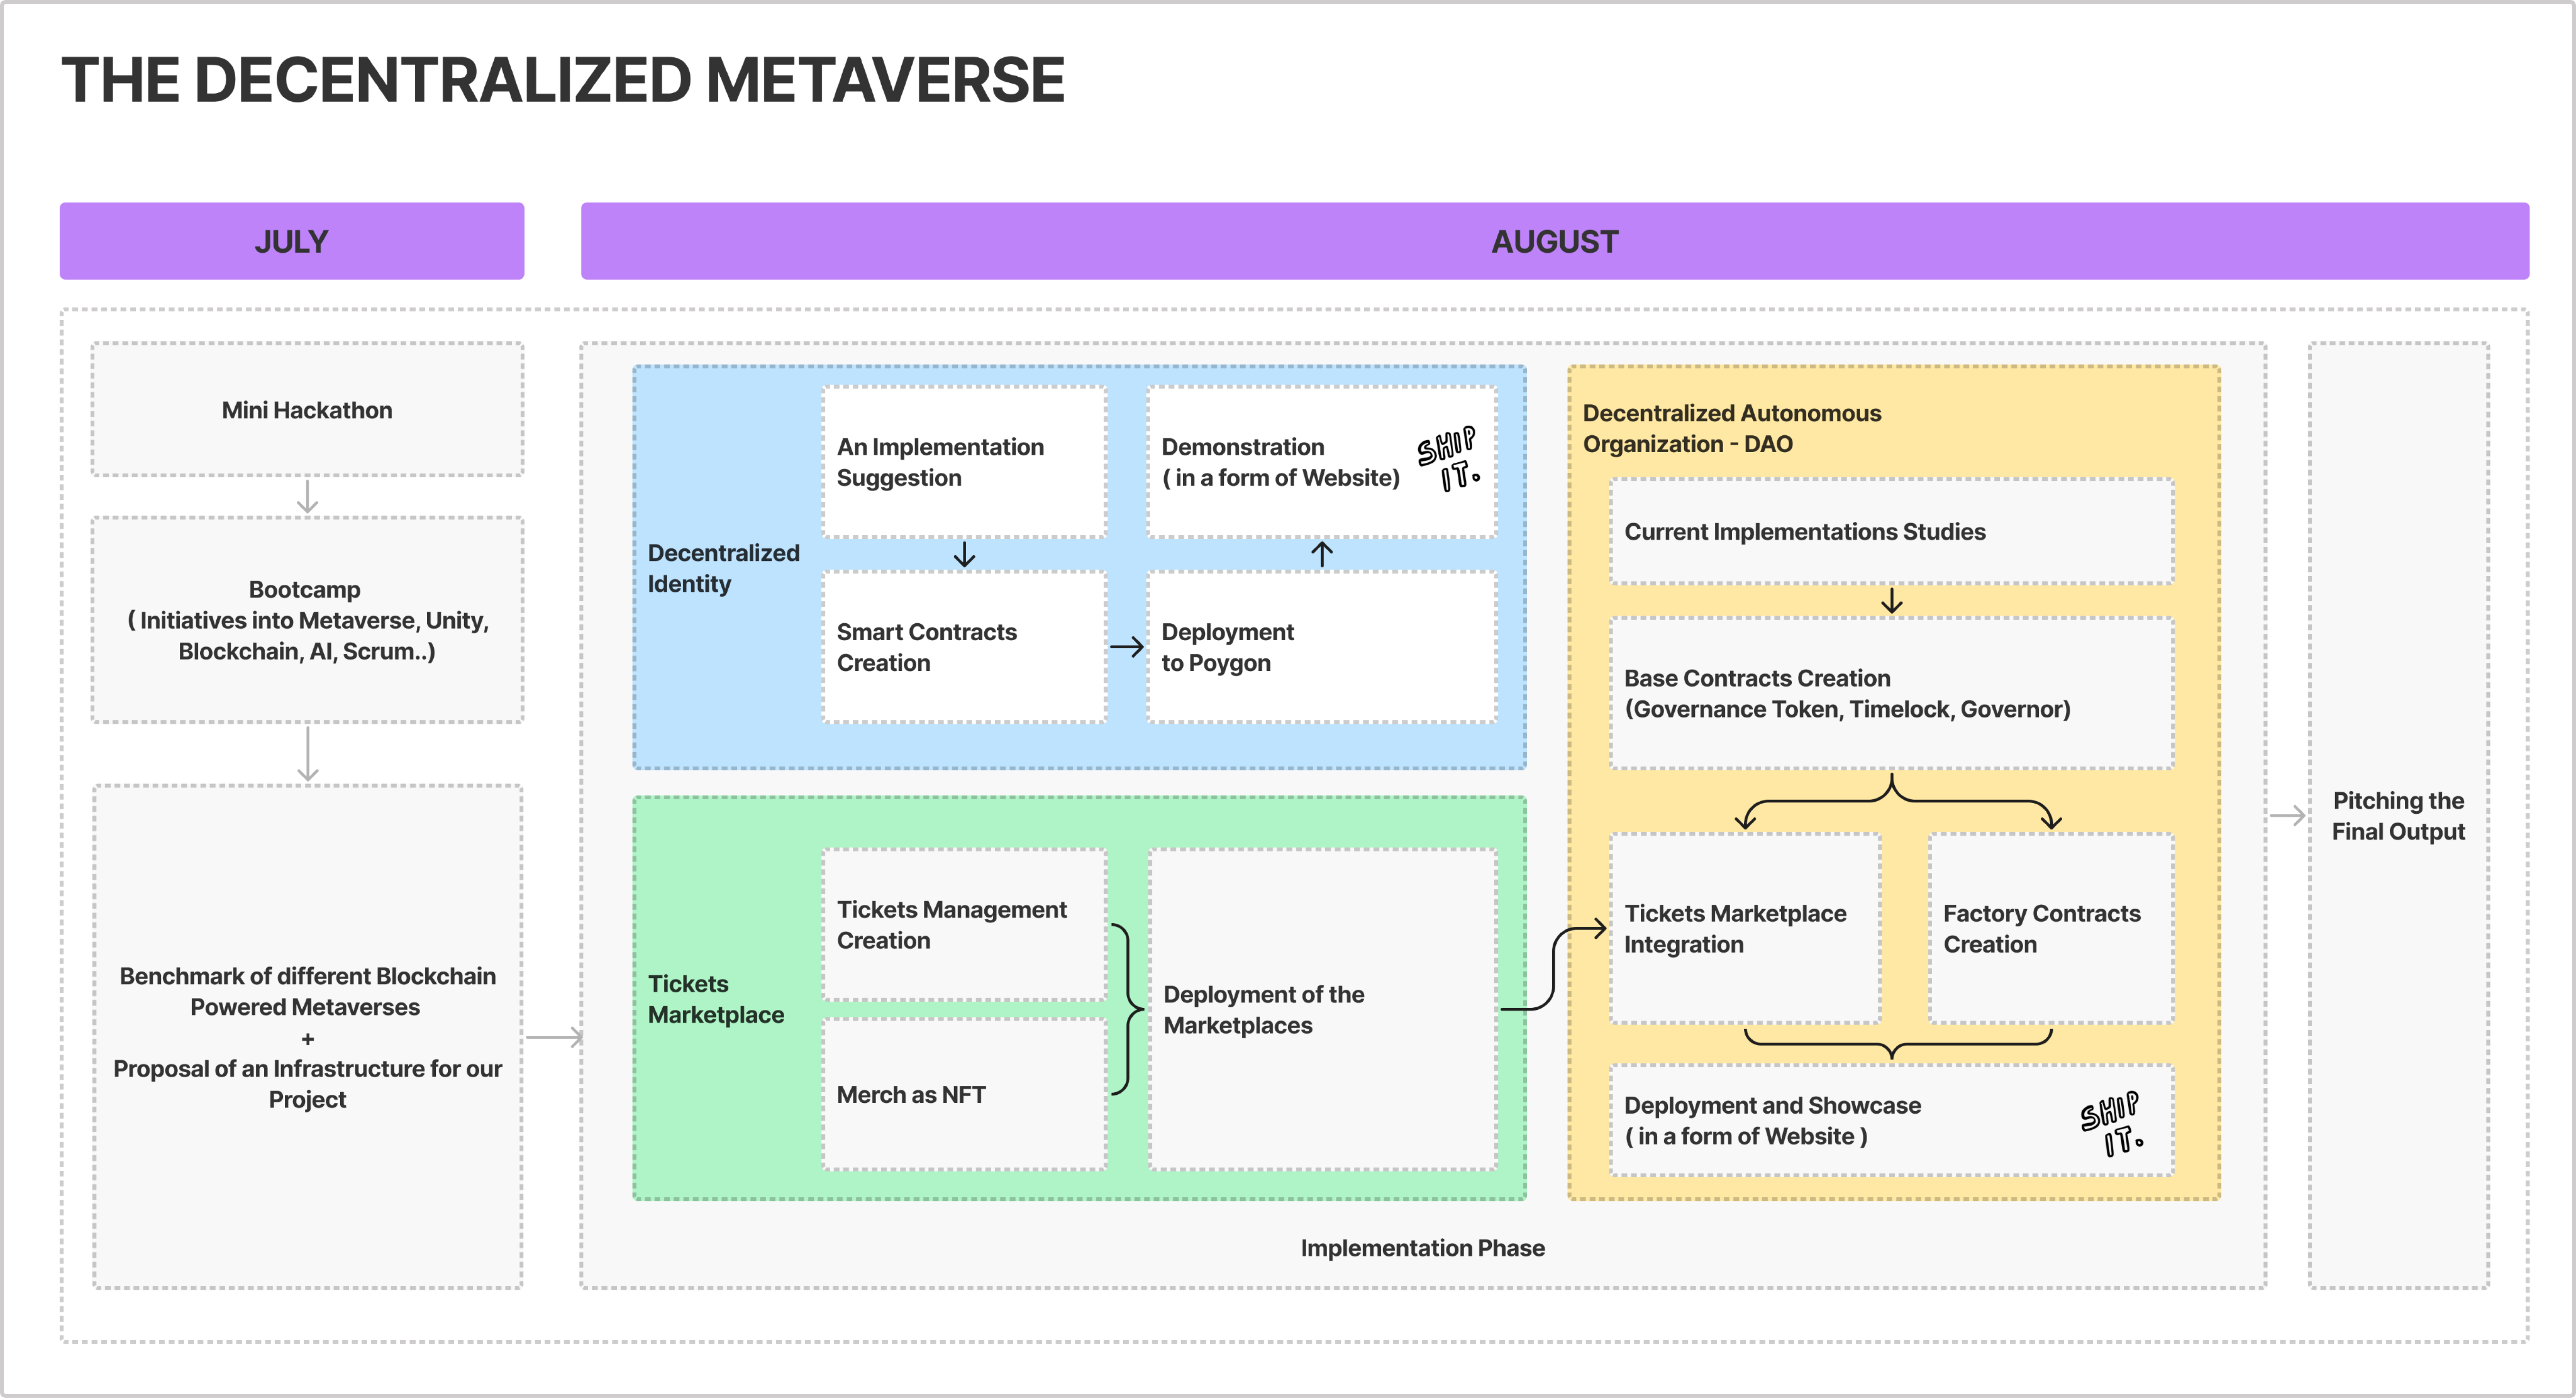
\includegraphics[width=1.5\textwidth]{assets/gantt.png}\\[0.1in]}



